\chapter{Einleitung}

\section{Aufgabe/Motivation}
Ziel des Versuchs war es, den grundlegenden Umgang mit dem Oszilloskop zu erlernen. Dazu gehörte das Kennenlernen der Bedienelemente, das Aufnehmen und Analysieren elektrischer Signale sowie das Verständnis der Messprinzipien. Das Oszilloskop dient in fast allen Bereichen der Elektronik als zentrales Werkzeug, weshalb die sichere Handhabung für weitere Anwendungen essenziell ist.

\section{Physikalische Grundlagen}
\cite{skript25}
Zunächst werden einige grundlegende Größen und Konzepte eingeführt, die für die weitere Analyse wichtig sind. Die Periodendauer $T$ eines Signals gibt die Zeit an, die eine vollständige Periode durchläuft, während die Frequenz $f$ durch
\begin{equation}
f = \frac{1}{T}
\label{eq:freq}
\end{equation}
definiert ist.  

Für Wechselspannungen werden mehrere Spannungsarten unterschieden. Die Spitze-Spitze-Spannung $U_\text{SS}$ gibt die Differenz zwischen dem maximalen und minimalen Spannungswert an. Der Effektivwert $U_\text{eff}$ ist die konstante Gleichspannung, die an einem Widerstand die gleiche Energie liefert wie die Wechselspannung. Für eine sinusförmige Spannung gilt:
\begin{equation}
U_\text{eff} = \frac{U_\text{SS}}{\sqrt{2}}.
\end{equation}

Wechselstrom (AC, alternating current) ändert periodisch Richtung und Betrag, während Gleichstrom (DC, direct current) zeitlich konstant bleibt.  

\section{Aufbau und Funktionsweise eines Oszilloskops}
Ein Oszilloskop dient der zeitlichen Darstellung elektrischer Signale. Analoge Oszilloskope nutzen einen Elektronenstrahl, der durch elektrische Felder auf einem Leuchtschirm abgelenkt wird. Das Eingangssignal steuert die vertikale Ablenkung, eine Sägezahnspannung die horizontale Ablenkung. Dies basiert auf den Bewegungsgesetzen geladener Teilchen im elektrischen Feld und Prinzipien der Elektronenoptik. Vorteil: kontinuierliche Darstellung, hohe Amplitudenauflösung.

Digitale Oszilloskope nehmen das Signal über einen Analog-Digital-Wandler (ADC) in festen Intervallen auf, speichern die Werte und stellen sie auf einem Bildschirm dar. Das Nyquist-Theorem bestimmt die minimale Abtastrate, um Signale korrekt zu rekonstruieren. Vorteile: Speicherung, mathematische Verarbeitung, Triggerung, digitale Analyse. Nachteil: begrenzte Auflösung durch diskrete Abtastwerte.
\begin{figure} [h!]
    \centering
        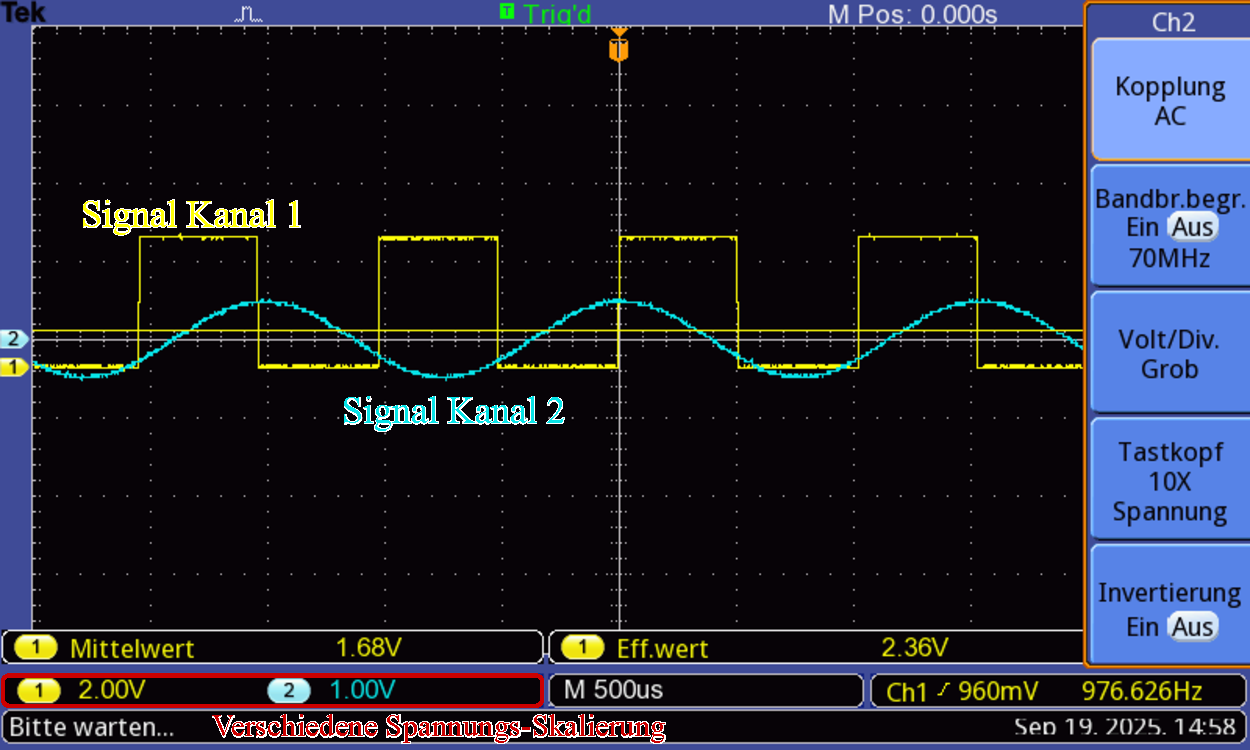
\includegraphics[width=0.45\textwidth]{img/25/2Kanal.pdf}
    \caption{Zwei verschiedene Signale gleichzeitig.}
\end{figure}


\subsection{yt-Betrieb}
Im yt-Betrieb wird Spannung gegen Zeit dargestellt. Das Signal wird am Eingang gedämpft, verstärkt, gefiltert und dann abgetastet. Die Abtastrate muss höher als die Signal-Frequenz sein, um Verzerrungen zu vermeiden. Die Bandbreite definiert die Frequenz, bei der ein sinusförmiges Signal auf 71\% seiner Amplitude abgeschwächt wird.
\begin{figure} [h!]
    \centering
        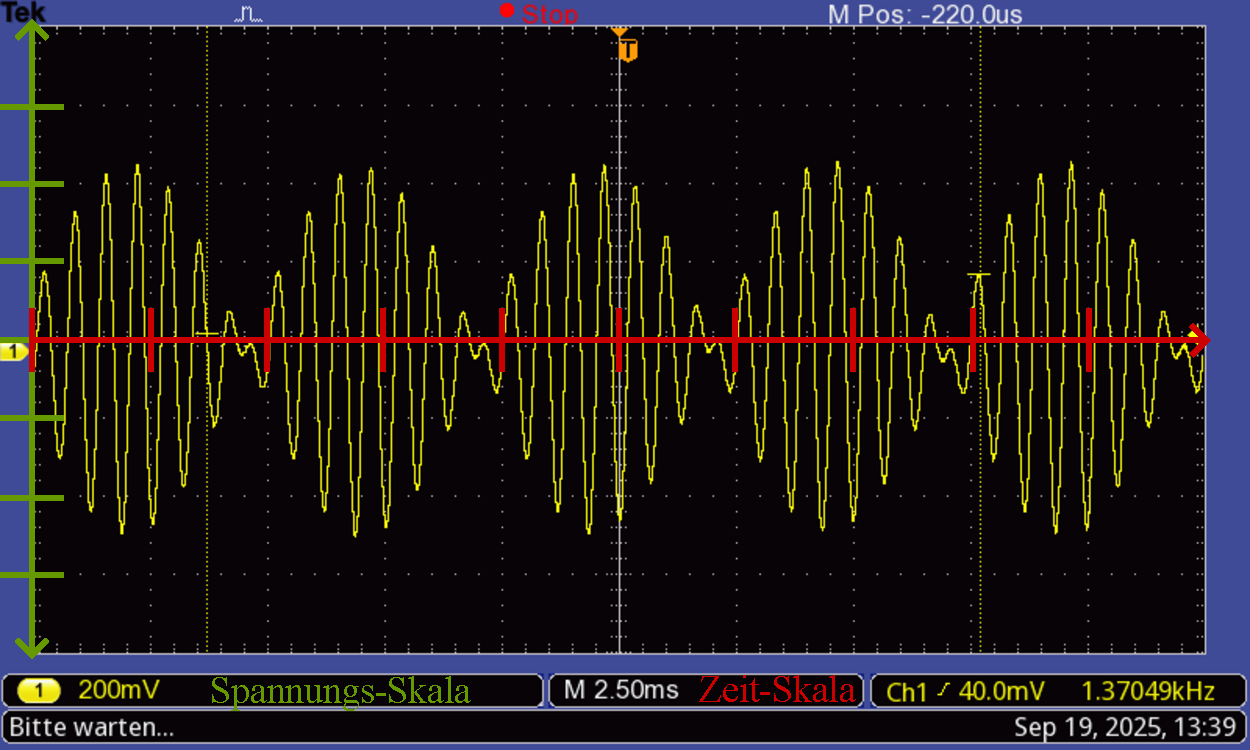
\includegraphics[width=0.45\textwidth]{img/25/yt-Achsen.pdf}
    \caption{Achsen klar visualisiert}
\end{figure}

\subsection{Triggerung}
Triggerung stabilisiert periodische Signale, verhindert Flackern und sorgt dafür, dass immer der gleiche Signalabschnitt dargestellt wird. Meistens wird eine Flankentriggerung verwendet, bei der ein Triggerlevel festgelegt wird, an dem das Signal abgebildet wird. Steigende oder fallende Flanken können gewählt werden.
\begin{figure} [h!]
    \centering
        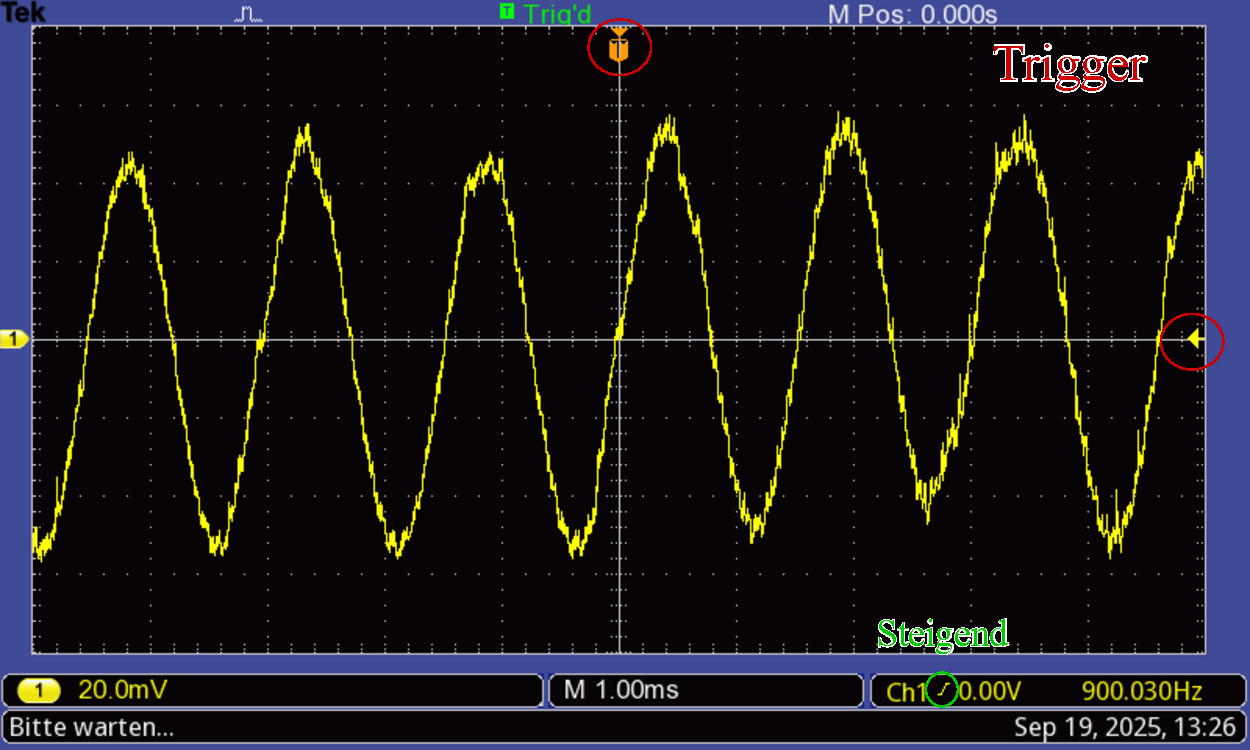
\includegraphics[width=0.45\textwidth]{img/25/Triggering.pdf}
    \caption{Visualisierung Triggering}
\end{figure}


\subsection{Bedienung}
Wichtige Funktionen sind die Eingangskopplung (AC, DC, Erde) sowie die vertikale und horizontale Skalenanpassung. AC-Kopplung filtert Gleichanteile, DC-Kopplung zeigt sie an. Die Erde-Position dient zur Nulljustierung.

\subsection{Reflexion auf Leitungen}
Ändert sich der Wellenwiderstand einer Leitung, wird ein Teil der Welle reflektiert. Der Wellenwiderstand $Z$ hängt von Induktivität $L'$ und Kapazität $C'$ pro Längeneinheit ab:
\begin{equation}
Z = \sqrt{\frac{L'}{C'}} \quad [\Omega].
\end{equation}
Offene Leitungen reflektieren ohne Phasensprung, kurzgeschlossene mit Phasensprung. Passender Abschluss eliminiert Reflexionen.

\subsection{Pulsweitenmodulation (PWM)}
PWM regelt Effektivspannung ohne Änderung der Betriebsspannung. Bei einer Impulsspannung $U_0$ ergibt sich Mittelwert $U_M$ und Effektivwert $U_\text{eff}$ über das Verhältnis von Pulsdauer $t$ zu Periodendauer $T$:
\begin{equation}
U_M = U_0 \frac{t}{T}, \quad
U_\text{eff} = U_0 \sqrt{\frac{t}{T}}.
\label{eq:spannungen}
\end{equation}
So kann man bspw. LEDs dimmen.
\begin{figure} [h!]
    \centering
        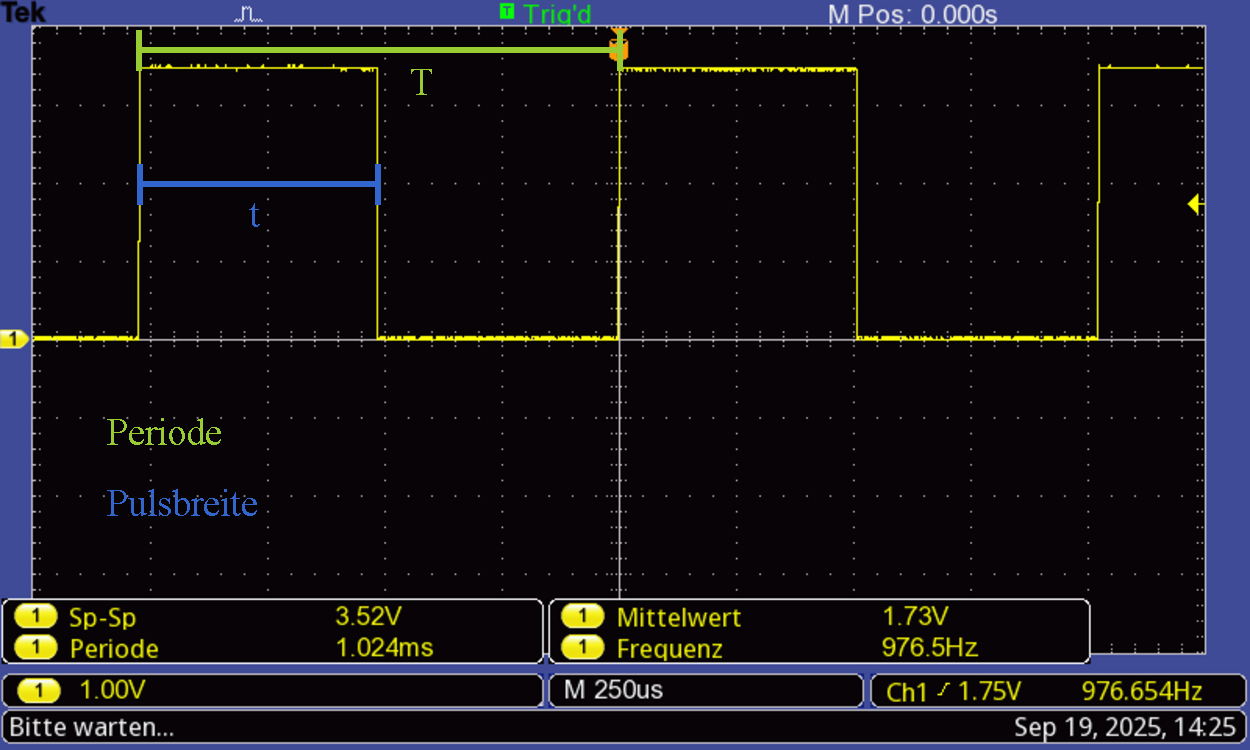
\includegraphics[width=0.45\textwidth]{img/25/PulsDef.pdf}
    \caption{Eingezeichet sind die Periode T und die Pulsbreite t.}
\end{figure}